\documentclass[11pt,a4paper]{article}
\usepackage[latin5]{inputenc}
\usepackage[english]{babel}
\usepackage{amsmath}
\usepackage{amsfonts}
\usepackage{amssymb}
\usepackage{graphicx,subfig}
\usepackage{placeins}
\usepackage{gensymb}

\author{Alexander Attinger, Yannic Kilcher}
\title{Report Blatt 7}

\begin{document}
\maketitle

\section{Excecise 1}
\paragraph{Image Rectification}
In the previous excercise sheet, we found a few matching points in corresponding stereo images and used them to calculate the fundamental matrix. Ideally, all the pixels of an image which have a corresponding pixel in the other image should be found and matched. This, of course is a very difficult task. It is made easier by the process of image rectification. In rectified images, corresponding pixels should all be in the same row. making the process of finding matches a lot easier. Luckily, OpenCV provides a function for rectification of images taken with uncalibrated cameras.

\section{Excercise 2}
The rectified images obtained in excercise 1 can now be used to calculate a disparity map. Binocular disparity is an importand depth clue in stereo vision. It describes the phenomenon that objects close to a pair of cameras or eyes for that matter, will have a bigger disparity than objects further away. We used a semi global block matching algorithm implemented in OpenCV to calculate the disparity in the different images. We were asked to try out different parameters. The results are shown in figures \ref{fig:3} and \ref{fig:4}.



\paragraph{Discussion}
Calculating the 3D coordinates of points with a disparity map is a different approach than what we discussed in the seminar, stratified reconstruction (the approach discussed in the Zisserman book). One of the advantages is the fact that it is not requiered to calculate the plane at the infinity. A disadvantage is the requirement, that the disparity only occurs in the horizontal direction, this, of course can be obtained by careful placement of the cameras and image rectification, nevertheless, it is at least in theory less general than stratified reconstruction. Also, the results we obtained are not very promising.

When small block sizes are used and the smootheness is not enforced, the resulting maps are very speckled and probably useless for further usage without processing. Maybe a median filter of some sort could help here. The second set of disparity maps are smoother, however, a lot of detail, which is still visible to our eyes in the first set of maps, is lost and edges are not straight.Perhaps the results of this algorithm can be improved by preprocessing images. Histogram equalization could increase contrast and facilitate matching of points, possibly improving both the estimate of $F$ and the disparity map. Foreground segmentation could be another useful trick. Usually, disparity vanishes when objects are distant enough from the cameras (exact value not known to us). So the resulting disparity seen for example in the upper regions of both the disparity map of the table scene and the street scene probably noise. Additionally, background objects are ususally out of focus (car scene) or homogenous (the back wall in the table scene), further reducing the quality of the matching and thus the resulting disparity map.



\begin{figure}
\centering
\subfloat[][View 1]{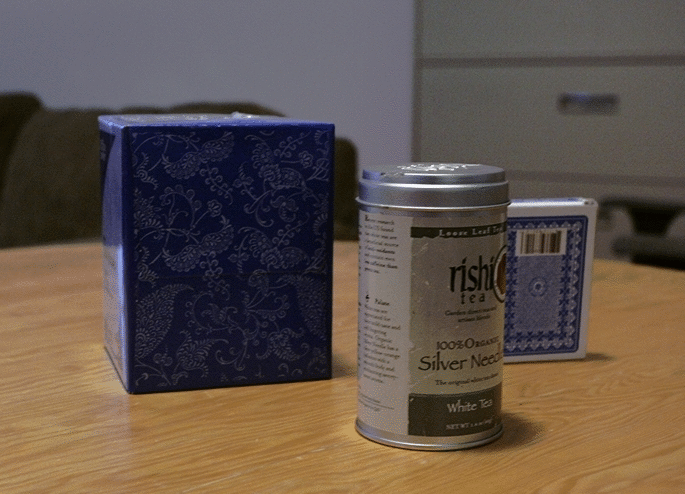
\includegraphics[scale=.25]{img/table1.png}}

\subfloat[][View 2]{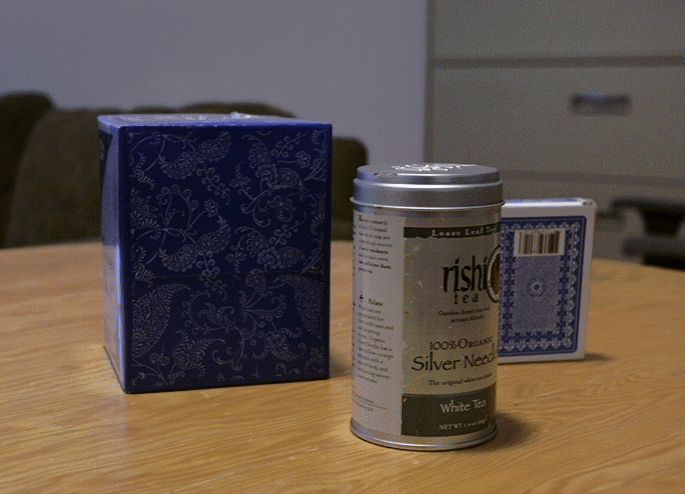
\includegraphics[scale=.25]{img/table2.png}}

\subfloat[][Rectified View 1]{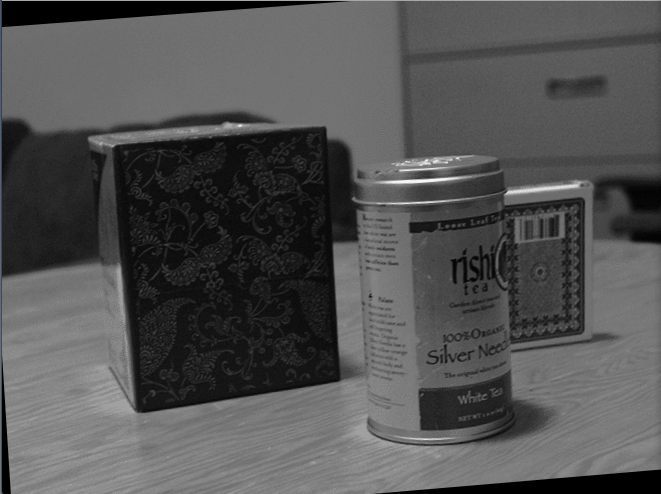
\includegraphics[scale=.25]{img/rectTable1.png}}

\subfloat[][Rectified View 2]{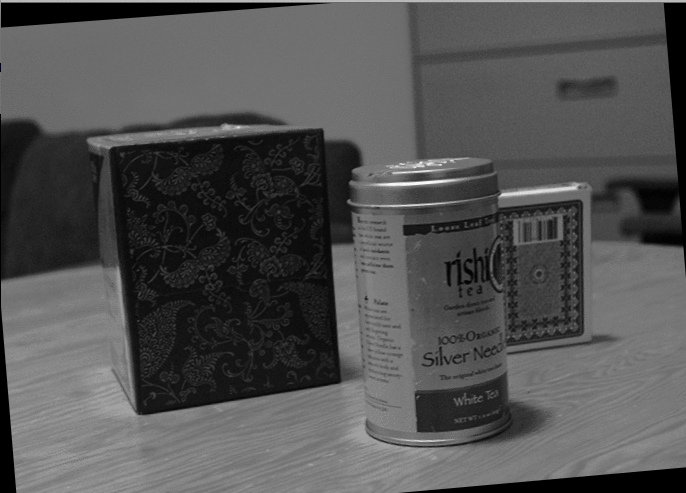
\includegraphics[scale=.25]{img/rectTable2.png}}

\caption{The two views of the table scene. From these two views, $F$ is calculated as described in the last report. The images are then rectified using $F$. The lower two images show the result of the rectification. It appears a little distorted compared to the original views, but much less so than the street scene (Figure \ref{fig:2}}%
\label{fig:1}
\end{figure}



\begin{figure}
\centering
\subfloat[][View 1]{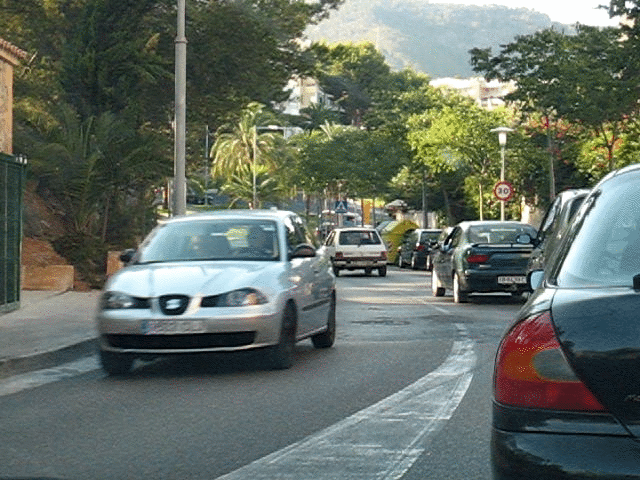
\includegraphics[scale=.25]{img/car1.png}}

\subfloat[][View 2]{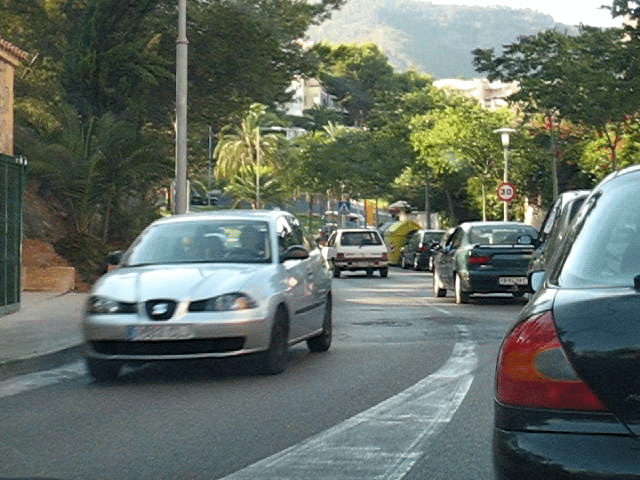
\includegraphics[scale=.25]{img/car2.png}}

\subfloat[][Rectified View 1]{\includegraphics[scale=.25]{img/rectcar1.png}}

\subfloat[][Rectified View 2]{\includegraphics[scale=.25]{img/rectcar2.png}}

\caption{The two views of the street scene. From these two views, $F$ is calculated as described in the last report. The images are then rectified using $F$. The lower two images show the result of the rectification. It appears very distorted compared to the original views.}%
\label{fig:2}
\end{figure}

\begin{figure}
\centering
\subfloat[][Disparity map 1]{\includegraphics[scale=.4]{img/disptable1.png}}

\subfloat[][Disparity map 2]{\includegraphics[scale=.4]{img/disptable2.png}}



\caption{The two disparity maps calculated using the semi global block matching algorithm implemented in OpenCV with two different parameter sets. With small block size and without smoothenes enforced (a), the map appears speckled, but for our eyes details are visible which disapear for larger block sizes and smootheness enforced.}%
\label{fig:3}
\end{figure}

\begin{figure}
\centering
\subfloat[][Disparity map 1]{\includegraphics[scale=.4]{img/dispcar1.png}}

\subfloat[][Disparity map 2]{\includegraphics[scale=.4]{img/dispcar2.png}}



\caption{The two disparity maps calculated using the semi global block matching algorithm implemented in OpenCV with two different parameter sets. With small block size and without smoothenes enforced (a), the map appears speckled, but for our eyes details are visible which disapear for larger block sizes and smootheness enforced.}%
\label{fig:4}
\end{figure}

\FloatBarrier



\end{document}
